\chapter{Results}\label{ch:results}

From the experiments described in chapter \ref{ch:experiments} a framework was created and tested in chapter \ref{ch:method}. 
The easy to use tools like iPerf3, Hping and BoNeSi are useful for quick tests. But when it comes to representative session based application testing these tools do not offer the solution for high speed networks. 
As these 'easy to use' tools all require the kernel to talk to the hardware. As described in section \ref{sub:dpdk}, DPDK is able to bypass the kernel and talk to the interface directly. Cores and memory needs to be allocated to generate traffic.  

\section{Infrastructure}
The network at 'company x' as it is visualized in figure \ref{fig:testenv} is a simplified representation.
The detailed infrastructure used during the real world test is displayed in figure \ref{fig:companyx} 
Since all the network hardware is redundant, the figure gets more complicated.
The server is connected to a data center layer that is spread over two physical locations and connected by DWDM.
To minimize the unnecessary traffic between the data centers on overlay technique is used.  
When traffic does not arrive at the destination, detailed measurements are needed at every device for every link to determine where the traffic gets dropped.  

\begin{figure}[] 
  \includegraphics[scale=0.4]{images/companyx.pdf}
  \caption{Detailed visualization of real world scenario.}
  \label{fig:companyx}
\end{figure}

\section{DPDK based}
Since none of the use cases require the 'easy to use' tools, simply due to the fact these tools did not hit the performance required for this research. 
The results of the DPDK based applications are explained during the use case performance tests on the real world scenario.
  
\subsection{pktgen}
Pktgen was used to get the limitations from the test hardware, it was already known that the maximum amount of pps is a hardware limitation inside the PCI Express Bus. 
The maximum link speed can be reached when packets of 400bytes are used. To get an idea of the throughput over the entire path from client to server. Pktgen is used to setup a UDP stream from the client to the server. 
The source IP address and port towards the destination IP address and port are the same. Since aggregated interfaces are used from the test switch to the router. The hashing algorithm in the switch made sure only one link was filled up by this test. 
Figure \ref{fig:surftest} shows a maximum throughput of 7 GB at 20:40. This was transported to company x and delivered to router1. From here it is important to know what lines are used to transport the traffic towards the firewall.
Figures \ref{fig:testrealusageae112} and \ref{fig:testrealusageae113} display the graphs of the traffic that went out of the interfaces connecting router1 to the firewall cluster and the links connecting the firewalls to the DCI switches inside the data center. The white gaps between send and received data, is traffic that got lost during the execution of the use cases.
   
\begin{figure}
  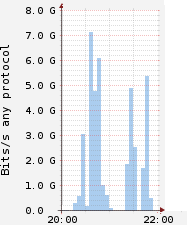
\includegraphics[scale=0.6]{images/test-link-usage.png}
  \caption{Bandwidth utilization of real world tests.}
  \label{fig:surftest}
\end{figure}

\begin{figure}
  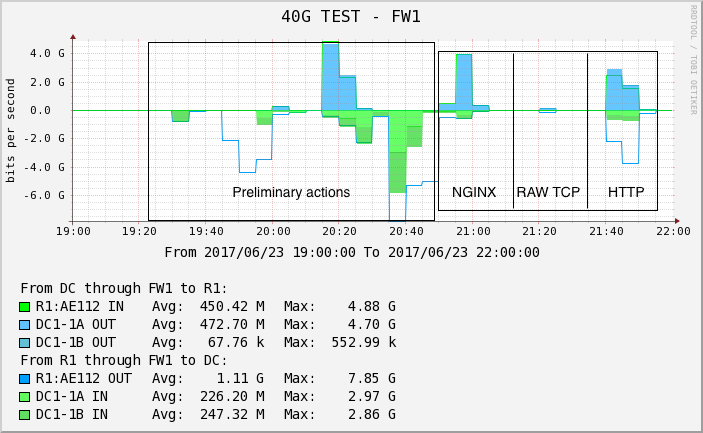
\includegraphics[scale=0.6]{images/real-ae112.png}
  \caption{Bandwidth utilization of links between router1, firewall1 and DC1.}
  \label{fig:testrealusageae112}
\end{figure}

\begin{figure}
  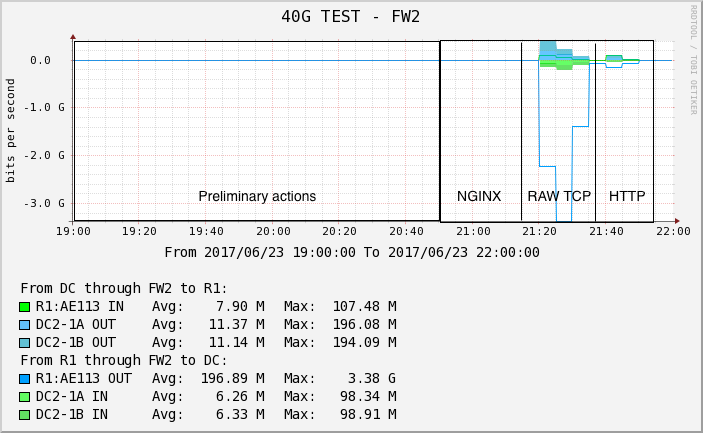
\includegraphics[scale=0.6]{images/real-ae113.png}
  \caption{Bandwidth utilization of links between router1, firewall2 and DC2.}
  \label{fig:testrealusageae113}
\end{figure}



% 20:42 - 20:50 PKTGEN UDP en TCP
% 20:54 - 21:00 WARP - NGINX
% 21:21 - 21:30 WARP - RAW TCP
% 21:42 - 22:00 WARP - HTTP

\subsection{WARP}
From the benchmark results performed on WARP in chapter \ref{ch:experiments} it is known WARP is capable of generating almost a Million sessions per second. WARP was used to retrieve a 500K file form an NGINX web server running on server A.
The file was placed on a RAM disk to make sure disk IO will not be the bottleneck of the performance tests. 
This test is executed on 20:50 and ran until 21:00. Request size increased every 90 seconds with an interval of 30 seconds between the tests.
Request sizes during this test: 64, 256, 512, 1024 and 2048 bytes. 
Figure \ref{fig:realnginx} displays that the amount of traffic leaving the server goes above 4Gb while only 0.6 Gb of requests are coming in. 
This matches the values shown in figure \ref{fig:testrealusageae112}. \\
Rate limiting at the NGINX server made sure nothing broke. The services got depleted at the machine, this made the service unavailable for other users.

\begin{figure}
  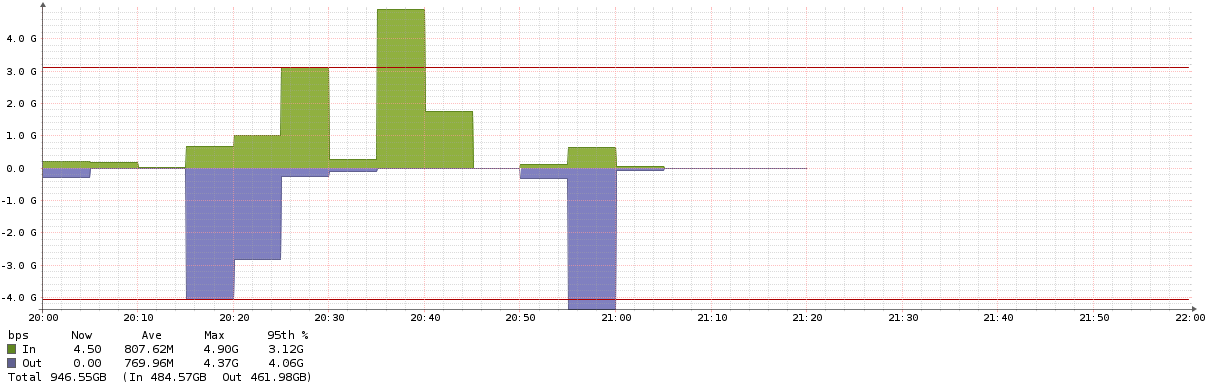
\includegraphics[scale=0.35]{images/real-nginx.png}
  \caption{Bandwidth utilization server A during NGINX test, measurements from servers perspective }
  \label{fig:realnginx}
\end{figure}


At 21:20 the next test is started. Generating a maximum amount of RAW TCP sessions from Client to Server both running WARP, Using 32GB memory and all cores to generate traffic.
Request and response sizes chosen for this tests are: 64, 256, 512, 1024 and 2048 bytes. 
Since WARP needs control of the interfaces, the server will not display any traffic on the interfaces. 
The measurements all came from the uplink and downlink interfaces of the Firewall. 
Sessions statistics where not registered due to logging problems in the firewall environment. 
Chapter \ref{ch:experiments} shows the benchmark of 1 million sessions per second are generated, no differences are shown at different packets sizes. 
Only 10\% of the link is utilized at the starting point of the test as displayed in \ref{fig:rawtcplink}. The graph in figure \ref{fig:testrealusageae112} doesn't display any traffic. 
The graph in figure \ref{fig:testrealusageae113} displays the load. When the test started, the active firewall crashed and a failover to the passive machine is the result. Log messages retrieved from connected routers also display BGP session failures from the former active firewall. 
This graph also displays the difference between traffic send from the Router to the firewall and the traffic received by the downstream switch. 
Input is 3Gb and output is in the range of 200 - 300 Mb. Clearly the firewalls are not capable of handling this amount of sessions. 
When the test was finished, the firewalls started to recover functionality. \\ 

The firewall environment was restored to the way it was in the beginning of the first test.
At 21:40 the last test is started between server and client, again both running WARP. Generating the maximum amount of HTTP sessions using 32Gb and all available cores.
Generating a GET request and responding with a 200-OK message. 
Message sizes for the tests are : 64, 256, 512, 1024 and 2048 bytes. Request and response size are equal. 
With the information from the benchmark in chapter \ref{ch:experiments} the limitations of client and server are known. 
From the tests at 21:20 it is known the machine will die when to many sessions per second come in. The same behavior is expected during this test.
Figure \ref{fig:testrealusageae112} displays the graph showing 4Gb going into the firewall and only 500Mb arriving at the other side.


